%%   This file is part of the APS files in the REVTeX 4 distribution.
%%   Version 4.0 of REVTeX, August 2001
%%
%%
%%   Copyright (c) 2001 The American Physical Society.
%%
%%   See the REVTeX 4 README file for restrictions and more information.
%%
%
% This is a template for producing manuscripts for use with REVTEX 4.0
% Copy this file to another name and then work on that file.
% That way, you always have this original template file to use.
%
% Group addresses by affiliation; use superscriptaddress for long
% author lists, or if there are many overlapping affiliations.
% For Phys. Rev. appearance, change preprint to twocolumn.
% Choose pra, prb, prc, prd, pre, prl, prstab, or rmp for journal
%  Add 'draft' option to mark overfull boxes with black boxes
%  Add 'showpacs' option to make PACS codes appear

% Edited by Camilla Harris Jan 2015
% For use by Camilla Harris, Akshat Mahajan
% in creating Lab Reports for 180c at UCLA
% this file and auxiliary files were retrieved from
% http://www-d0.fnal.gov/Run2Physics/WWW/templates/
% on Jan 19 2015

\documentclass[aps,prl,nofootinbib,twocolumn,superscriptaddress,groupedaddress]{revtex4}  % for review and submission
%\documentclass[aps,preprint,superscriptaddress,groupedaddress]{revtex4}  % for double-spaced preprint
% CAMILLA: I removed the PACS functionality
\usepackage{graphicx}  % needed for figures
	%if using postscript files compile with XeLaTex
\usepackage{dcolumn}   % needed for some tables
\usepackage{bm}        % for math
\usepackage{amssymb}   % for math
\usepackage[export]{adjustbox}
\usepackage{array}
\usepackage{multirow, bigdelim}

% avoids incorrect hyphenation, added Nov/08 by SSR
\hyphenation{ALPGEN}
\hyphenation{EVTGEN}
\hyphenation{PYTHIA}

\begin{document}
\title{Charge Density Waves in NbSe$_{3}$}
\input author_list.tex        % includes institutions and visitors
\date{\today}

\begin{abstract}
We present the results of measuring the properties of an NbSe$_{3}$ crystal (a charge-density wave system) as a function of electric field and temperature using a conventional four-probe measurement. The Peierls transition temperatures are 132.23 $\pm$ 9.95 K and 54.89 $\pm$ 1.52 K. Our threshold electric field values $E_{T}$ are 10.40 mV/cm at 45 K, 8.64 mV/cm at 47 K and 13.80 mV/cm at 55 K - not in agreement with reported values in the literature. We explore possible reasons for this in this paper.
\end{abstract}

\maketitle

\section{Background Information}

Niobium triselenide (NbSe$_{3}$) is among the few materials known to demonstrate a transition from conductor to an insulator state at low temperatures owing to what is known as a sliding charge density wave effect. The root cause of this behaviour stems from Peierls instability, where a periodic applied electric field of magnitude $V_{k_{f}}$ and wavenumber $k_{f}$ leads to spatial wavelike lattice distortions (a so-called charge-density wave). The effect of this is to open a band gap $\Delta = 2 V_{k_{f}}$ at the Fermi energy $E_{F}$. At room temperature, the surrounding thermal energy far exceeds the value of this band gap, allowing easy excitations to states above the band gap - at these temperature ranges, niobium triselenide behaves approximately like a conductor. At low temperatures, however, this behaviour is much less pronounced, and in these cases niobium triselenide begins to behave like an insulator with a large and well-defined band gap centered around the Fermi energy following a second-order phase transition at a particular temperature.

Curiously, as temperature is continuously lowered, niobium triselenide undergoes not one, but \textit{two} transition temperatures - in other words, it demonstrates a transition back to the conducting state from an insulating state and then back again to an insulating state from this second conducting state. This can be attributed to the opening of multiple band-gaps for different energy bands at much lower temperatures, reducing the conductivity by a much larger fraction.

In this paper, we reproduce this resistivity vs. temperature behaviour of NbSe$_{3}$ and identify the two Peierls transition temperatures $T_{P1}$, $T_{P2}$. As transition temperatures depend somewhat on the experimental setup, our method of identifying the two temperatures was to find the two global peaks in the graph of $\frac{d \ln  (R)}{d \left(\frac{1}{T}\right)}$ vs. $T$ - a method justified by theoretical estimations of the temperature sensitivity of resistance. A conventional four-wire resistance measurement was undertaken to this effect. A long thin strand of NbSe$_{3}$ was attached to a voltmeter with conventionally large resistance that measured the voltage $V_{s}$ across the sample. An alternating current of constant magnitude $I_{AC}$ throughout the circuit was applied across the sample, and its resistance was calculated using the formula

\begin{equation}
R = \frac{V_{s}}{I_{AC}}
\end{equation}

A cryocooler employing liquid helium and a heater was used to control temperature. Measurements were taken of both the sample's actual temperature and the temperature of a point some distance away, where the cryocooler actually operated upon - the former was called the \textsl{sample temperature} and the latter the \textsl{control temperature}. We chose to measure both the control and the sample temperature simultaneously in order to capture discrepancies between the crycooler's action and the actual sample temperature. We took three runs for the temperature, each time sweeping from close to 20 K to about 200 K. For the purposes of this experiment, a large amplitude $I_{AC}$ of the AC current - 5 $\mathrm{\mu}$A - was applied to the second and third, while 0.1 $\mathrm{\mu}$A was applied to the first. 

Related to the phenomenon of the sliding charge density wave is the behaviour of NbSe$_{3}$ under large electric fields. At a particular temperature, the resistance remains roughly constant, indicating a pinning of the sliding charge density wave  (in other words, the phase of the wave is fixed) - however, a sufficiently large electric field past a threshold $E_{T}$ is capable of depinning this charge density wave, and thereby prompting an abrupt fall in the resistance as the phase changes and electrons are `transported' through the medium. One can measure this effect by charting a current vs. applied voltage graph as well as by measuring differential resistance.

We employed the following setup: alternating current with a large DC bias was allowed to pass through the sample, connected in series with a resistor whose value is already known. An external voltage was generated over the sample, and the corresponding current that passed through the sample was recorded by measuring and tuning the voltage across the resistor. The DC component of the current allowed us to estimate the current vs. applied voltage of the sample, whereas the AC component could be used to resolve the sample's differential resistance as a function of applied voltage. All efforts were made to keep temperature roughly constant. In an attempt to discern the influence of temperature on the threshold electric field, we made three measurements near the lower transition point, namely at 45 K, 47 K and 53 K. The applied voltage across the resistor ranged from 0 - 10 mV in steps of 0.1 mV. 

\section{Results}
The corresponding graphs display our results. Tables that offer quantitative precision follow thereafter.
\onecolumngrid

\begin{center}
\begin{figure}[h]
\centering
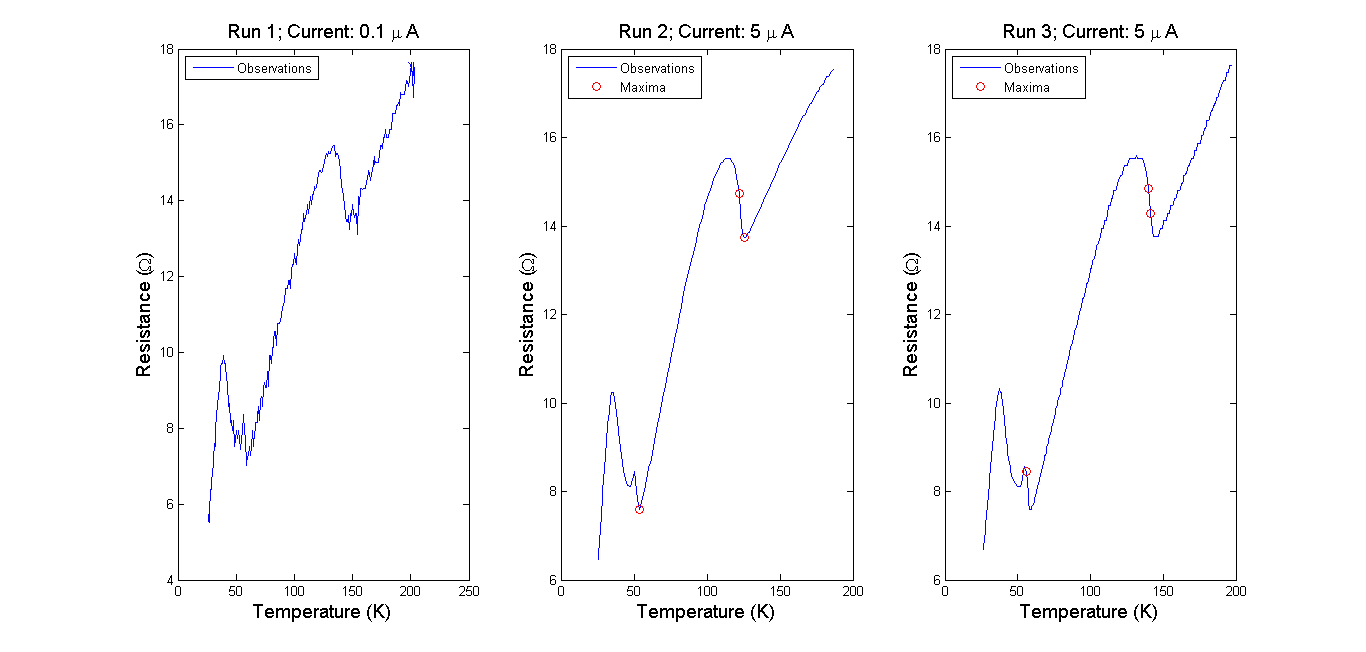
\includegraphics[scale=0.5]{../Analysis/ResistivitiesVersusTemperature.png} 
\caption{Resistance vs. temperature graphs for the sample NbSe$_{3}$.}
\end{figure}

\begin{figure}[h]
\centering
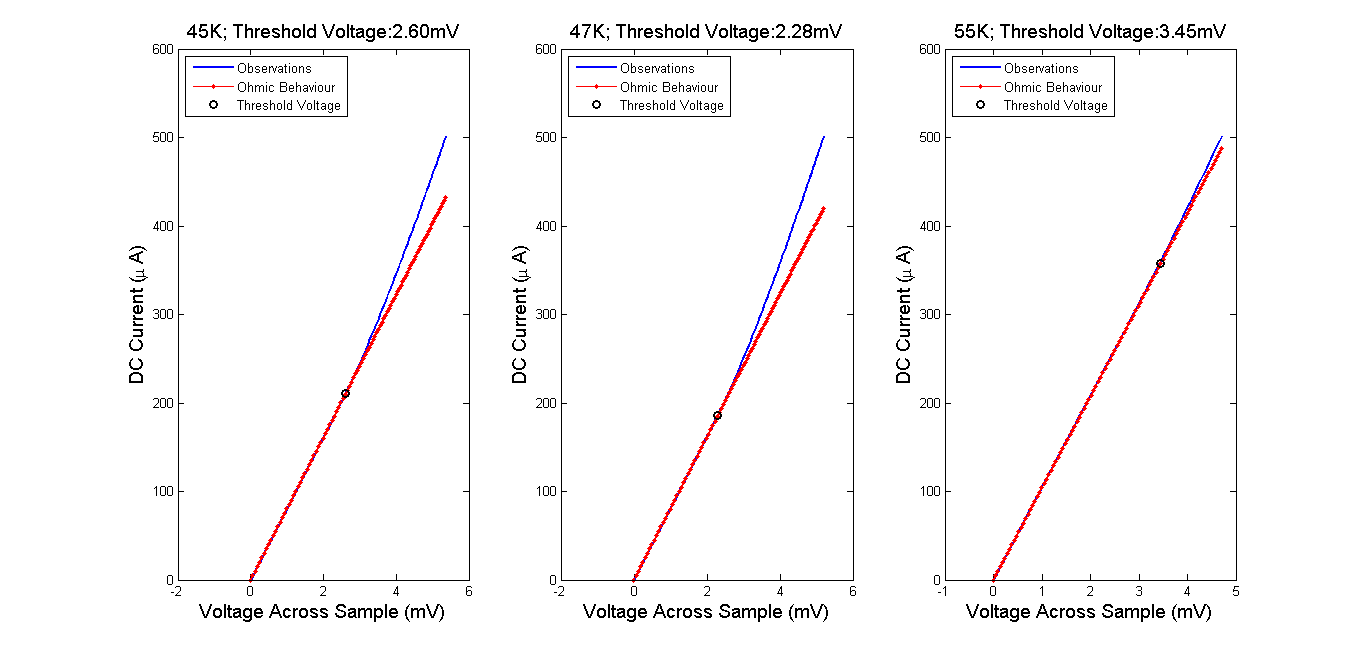
\includegraphics[scale=0.5]{../Analysis/DCCurrentVersusVoltage.png} 
\caption{DC current vs. voltage graphs for the sample NbSe$_{3}$. The red line indicates the expected Ohmic behaviour extrapolated from the first two points of observation (from 0 mV onwards). The existence of a gap between observations (blue) and the Ohmic curve clearly indicates that the resistance is changing.}
\end{figure}
\end{center}

\twocolumngrid

\noindent The red points in Fig. 1 indicate the points of local maxima in $\frac{d \ln  (R)}{d \left(\frac{1}{T}\right)}$ vs. $T$. Points were algorithmically chosen by ordering the maxima in decreasing order of height - three are displayed instead of two as it was found that points near the higher transition temperature were also large peaks; we attribute this to noise near the true upper transition temperature, and take the average of the points closest to each other. Run 1 has no peaks displayed - the signal-to-noise ratio was so low that the lower transition temperature signal was the tenth largest maxima, rather than the third or second. We choose to regard it as a bad run, and confine our attention to runs 2 and 3 instead where the signal-to-noise ratio is much higher. 

The threshold voltages in Fig. 2 were derived by first binning the current to reduce the amount of noise (averaging every five values), and then by plotting the resistance (obtained as the inverse of the slope). We chose the point preceding the most negative slope in the resistance curve as our threshold voltage value, on the basis that a significant fall in resistance will be markedly more prominent than those due to random noise. The possible errors and the validity of the assumption involved in this approach are discussed in the following section. 

\begin{table}[h]
\caption{\label{tab:table1} A table listing the temperatures of the maxima found in $\frac{d \ln  (R)}{d \left(\frac{1}{T}\right)}$ vs. $T$. All temperatures and derived quantities are in units Kelvin.}
\begin{ruledtabular}
\begin{tabular}{p{1.5cm}p{1.5cm}p{1.5cm}p{1.5cm}}
Run Number& Temperature of Maxima & Averaged Temp. & Standard Deviation\\
\hline
2 & 125.40 & \rdelim\}{4}{*}[132.23] & \multirow{4}{*}{9.95}\\
2 & 122.03 & &\\
3 & 140.03 & &\\
3 & 141.48 & &\\
2 & 53.81 & \rdelim\}{2}{*}[54.89] & \multirow{2}{*}{1.52}\\
3 & 55.97 & &\\
\end{tabular}
\end{ruledtabular}
\end{table}

\begin{table}[h]
\caption{\label{tab:table2} A table listing the threshold electric fields in Figure 2.}
\begin{ruledtabular}
\begin{tabular}{p{2cm}p{2cm}p{2cm}p{2cm}}
Temperature (K) & Threshold Voltage (mV) & Sample Length (cm) & Threshold Electric Field (mV/cm)\\
\hline
45 & 2.60 & 0.25 & 10.40\\
47 & 2.28 & 0.25 & 9.12\\
55 & 3.45 & 0.25 & 13.80\\
\end{tabular}
\end{ruledtabular}
\end{table}

\onecolumngrid

\begin{center}
\begin{figure}[h]
\centering
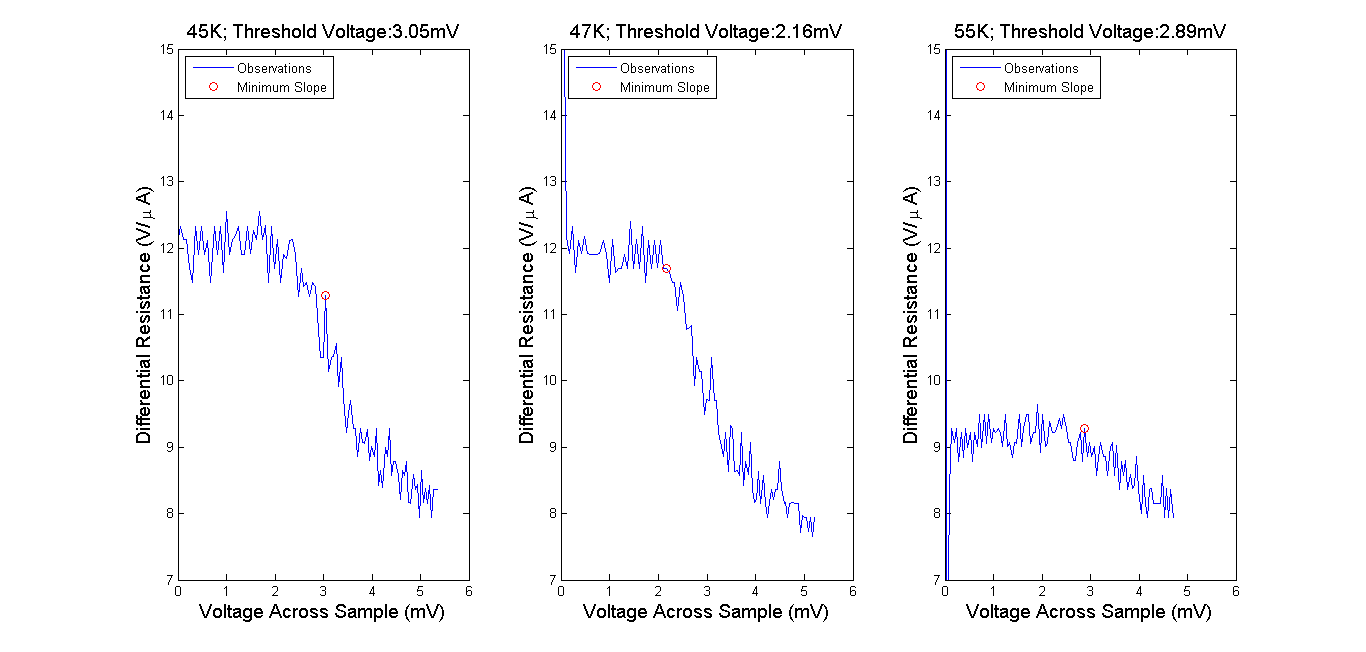
\includegraphics[scale=0.5]{../Analysis/../Analysis/ACCurrentVersusVoltage.png} 
\caption{Differential resistance of NbSe$_{3}$ vs. applied voltage across sample at different temperatures}
\end{figure}
\end{center}

\twocolumngrid

\begin{table}[h]
\caption{\label{tab:table3} A table listing the threshold electric fields in Figure 3.}
\begin{ruledtabular}
\begin{tabular}{p{2cm}p{2cm}p{2cm}p{2cm}}
Temperature (K) & Threshold Voltage (mV) & Sample Length (cm) & Threshold Electric Field (mV/cm)\\
\hline
45 & 3.05 & 0.25 & 12.2\\
47 & 2.16 & 0.25 & 8.64\\
55 & 2.89 & 0.25 & 11.56\\
\end{tabular}
\end{ruledtabular}
\end{table}

\noindent The threshold voltages in Fig. 3, marked by red circles, were determined by choosing those points preceding the most negative slope in the data. This is in line with the hypothesis that the phase transition is accompanied by a sharp decrease from roughly constant differential resistance. For the differential measurements at temperatures 47 K and 55 K, we exclude the first two points from analysis as they are significant outliers and can be attributed to random error.

\section{Analysis}
\noindent Here, we discuss potential sources of error and their impact on our results. Firstly, we note that all three sample runs in Fig. 3 and Fig. 2 were collected with AC current amplitude of 0.1 $\mu$A, and therefore that the signal has a correspondingly large amount of random noise. The approach used to calculate threshold fields with the differential measurement resistance is different from the approach used in the current-voltage measurement because of this - since low signal-to-noise ratio contaminates everything but it is impossible to distinguish noise from signal, we are forced to take two different approaches in the hope that they will present more clarity than just one method with the same consistent biases repeated throughout. In other words, we are trying to reduce the amount of error involved overall by contrasting two approaches to the same thing. While both measurements involve identifying the threshold voltage as the point preceding the most negative slope in the resistance vs. voltage data, the DC resistance approach explicitly involves noise reduction by first taking the average of every five consecutive values of current - the AC resistance does not do this, and so we are able to compare and contrast our results across two approaches.

One significant source of systematic error that stems from this is the possibility of incorrectly choosing the threshold voltage from the differential resistance measurements. We originally chose the threshold voltage by picking the point preceding the most negative slope - however, if slopes due to random fluctuation can have values that are comparable to the `true' negative slope (corresponding to the actual transition), then we may have incorrectly chosen a slope that is actually due to random fluctuations than to our true transition. By making the reasonable assumption that the distribution of slopes is Gaussian, we can estimate the probability that our chosen negative slope can be reproduced by Gaussian fluctuations by calculating the $z$-score of our chosen negative slope. The results of this investigation can be seen in Table IV.

\begin{table}[h]
\caption{\label{tab:table3} Calculated probability of occurrence $P$ of slope value from a Gaussian distribution of listed mean and standard deviation $SD$. Mean and SD were calculated from raw data. Slope values used here are the values used to derive threshold voltage from Fig. 3. Slope, mean and SD have units $\mu\Omega$/mV.}
\begin{ruledtabular}
\begin{tabular}{cccccc}
Temp. & Slope & Mean & S.D. & Z-Score & P \\
45 K & -1.7385 & -0.5341 & 4.0502 & 0.2974 & 76\%\\
47 K & -2.1181 & -0.0723 & 0.8272 & 2.4731 & 1.3\%\\
55 K & -1.4914 & -0.4198 & 4.9415 & 0.2169 & 82\%\\
\end{tabular}
\end{ruledtabular}
\end{table} 

\begin{table}[h]
\caption{\label{tab:table3} Calculated probability of occurrence $P$ of slope value from a Gaussian distribution of listed mean and standard deviation $SD$. Mean and SD were calculated from raw data. Slope values used here are the values used to derive threshold voltage from Fig. 2. Slope, mean and SD have units V/$\mu$A. There is a strong component of bias acting on these values.}
\begin{ruledtabular}
\begin{tabular}{cccccc}
Temp. & Slope & Mean & S.D. & Z-Score & P \\
45 K & -0.0023 & -0.0008 & 0.0007 & 1.8281 & 6.7\%\\
47 K & -0.0026 & -0.0009 & 0.0008 & 1.9245 & 5.4\%\\
55 K & -0.0008 & -0.0002 & 0.0003 & 1.9799 & 4.7\%\\
\end{tabular}
\end{ruledtabular}
\end{table} 

From Table IV, we can see that there is a high probability that we've chosen a slope due to random fluctuations in the signal at temperatures 45 and 55 K. The probability of randomly generating the slope chosen at 47 K is sufficiently low (less than 5\%, the standard significance level) as to reject the hypothesis that it is due to a random process. We therefore express some confidence in the accuracy of our result for a temperature of 47 K, and significantly less confidence in the accuracy of our $E_{T}$ measurements at other temperatures from the differential resistance measurement. In the future, much higher signal-to-noise ratios - the underlying cause of this error - can be achieved by raising the amplitude of the AC current up to 5 $\mu$A, leading to improvement upto 50 times.

We apply a similar test for our threshold voltages as derived from our DC measurements - the results are presented in Table V. While initial examination of Table V may lead to the conclusion that our results are robust, it is important to remember that there is a strong bias acting on the values returned. In particular, by averaging every five data points in our current, we have explicitly reduced the effect of noise. Since our goal was to estimate the likelihood of our chosen slope being generated by noise, it should not be surprising that the chosen negative slopes have high $z$-scores. Thus, the probabilities of occurrence as returned in Table V should not be interpreted in favour of or against our methodology. We leave the probabilities of occurence here, however, alongside a plot of our binned resistance vs. voltage in Fig. 4 for comparison with Fig. 2 to facilitate estimation of bias at a later date.

Choosing which of the two approaches - the approach used in the differential resistance measurement and the approach used in the DC resistance measurement - is a better estimate of the threshold field is not straightforward. Unlike the differential resistance measurement, the DC resistance measurement does not allow for strong analysis of error - however, two of the three values in the AC resistance measurement have been shown to have a high chance of being random fluctuation. We decide on the following compromise: for 45 K and 55 K, the threshold field is given by the corresponding DC measurement, whereas, for 47 K, the threshold electric field is given by the corresponding AC measurement. Our results are collected and presented in Table VI.

\begin{table}[h]
\caption{\label{tab:table3} Final threshold electric field values}
\begin{ruledtabular}
\begin{tabular}{ccc}
Temp. & Units & $E_{T}$ \\
\hline
45 K & mV/cm& 10.40 \\
47 K &mV/cm & 8.64 \\
55 K & mV/cm& 13.80\\
\end{tabular}
\end{ruledtabular}
\end{table} 

The reported values\cite{et} of $E_{T}$ at approximately 47 K are 4.4 mV/cm and 31.7 mV/cm at 50.1 K. Our results, for both the AC and DC resistance approaches and overall, do not appear to match - however, we note that these reported values were derived from a least-squares fit with multiple parameters to experimental data\cite{et}, and not using the approaches outlined. We recognise, however, that our observed values are not consistent with the proposed temperature-dependence of the threshold field as exponentially decaying\cite{ong}. 

Following Ong and Monceau\cite{ong}, we denote $\alpha$ as the temperature-dependent fraction of the Fermi surface destroyed by charge-density wave formation at the transition temperature. The parameter $\alpha$ obeys the following relationship with resistance\cite{ong}:

\begin{equation}
\alpha = \frac{\frac{1}{R(E \rightarrow 0)}}{\frac{1}{R(E \rightarrow 0)} + \frac{1}{R(E \rightarrow \infty)}} 
\end{equation}

Given that that the lower transition temperature is around 54 K, we can use our DC measurements at 55 K to roughly approximate our value for $\alpha$. We calculate the slope $\left( = \frac{1}{R}\right)$ from our DC measurements at $V = 6$ mV and at $V = 0$ mV and substitute accordingly:
$$
\alpha = \frac{\frac{1}{R(E \rightarrow 0)}}{\frac{1}{R(E \rightarrow 0)} + \frac{1}{R(E \rightarrow \infty)}} = \frac{105.2034}{105.2034 + 116.7647} = 0.474
$$

Thus, the change in the Fermi surface is approximately 48\% from its original value at the lower transition temperature.

\onecolumngrid

\begin{center}
\begin{figure}[b]
\centering
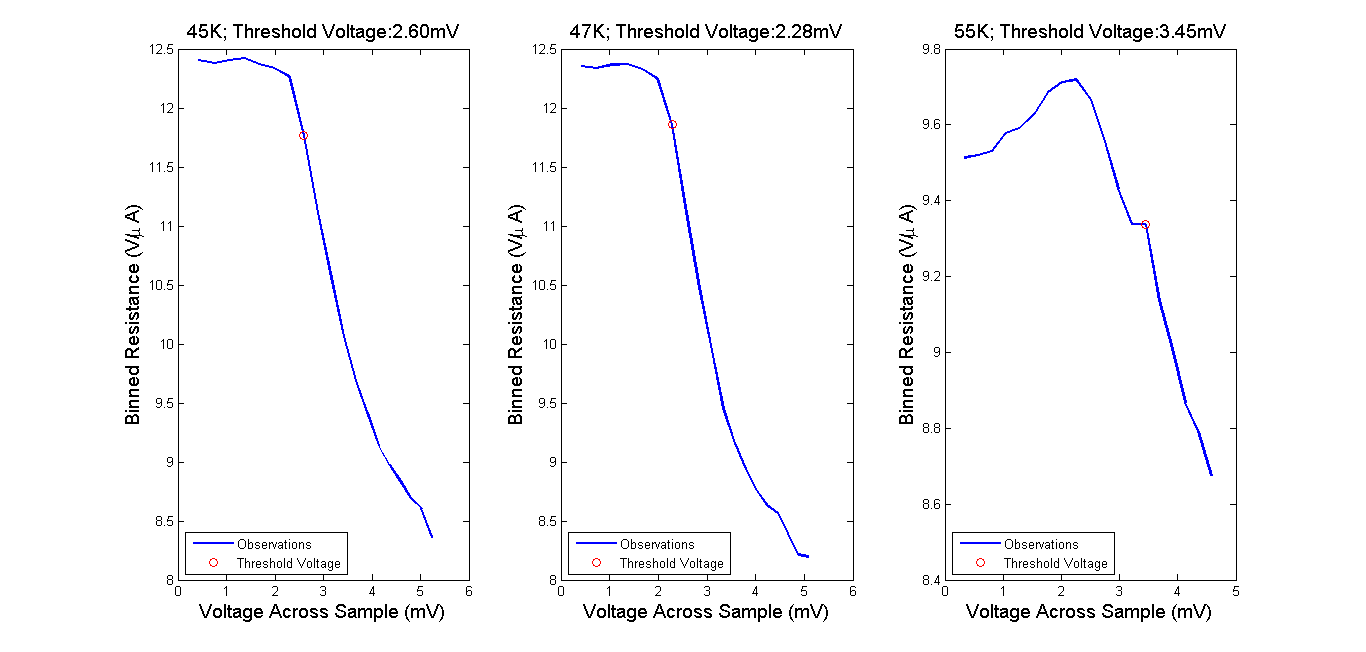
\includegraphics[scale=0.5]{../Analysis/../Analysis/DCResistanceVersusVoltage.png} 
\caption{Resistance versus applied voltage for NbSe$_{3}$, derived by inverting the slope of the binned values of current in Fig. 2}
\end{figure}
\end{center}

\newpage
\twocolumngrid

The effect of increasing temperature on the I-V characteristics appears to be straightforward from Fig. 2 - as temperature increases, divergence from Ohmic behaviour becomes much less prominent. This is in keeping with our expectation that, at higher temperatures, NbSe$_{3}$ behaves like a metal. Whether this trend undergoes an abrupt change at the higher transition temperature will require further work, but \textit{a priori} it appears that this trend holds for the few values we have seen.

Finally, we address the question of whether our AC measurements have a good match with our DC measurements i.e. whether one is a good representation of the other, or, in other words, if they are describing the same data. We reconstructed the current vs. voltage behaviour using our differential resistance - the results can be seen in Fig. 5. We can see that, for low fields, there is reasonable agreement between the reconstructed and DC-measured values, but, for large fields, they start to diverge.  

\onecolumngrid

\begin{center}
\begin{figure}[t]
\centering
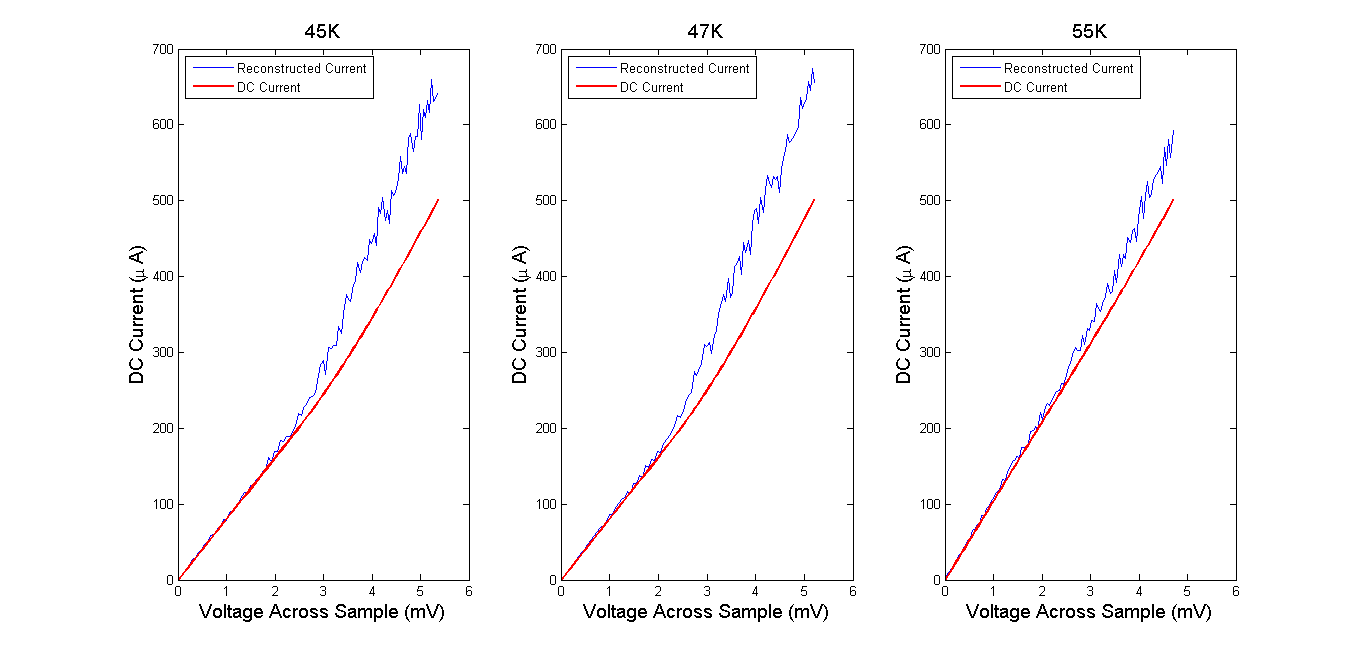
\includegraphics[scale=0.5]{../Analysis/../Analysis/ReconstructedCurrent.png} 
\caption{Reconstructed current vs. voltage graph frm AC measurements.}
\end{figure}
\end{center}

\twocolumngrid

\section{Conclusion}

In conclusion, we report that there is significant room for improvement in the experiments that involve measurement of the threshold electric field $E_{T}$. In particular, higher AC amplitude of current can drastically improve the resolution of our signal. Our transition temperature values have reasonably good agreement with the accepted values\cite{ong} of the transition temperature for NbSe$_{3}$ (144 K and 59 K).
\begin{thebibliography}{2}

 \bibitem{ong}
    \textit{Anomalous transport properties of a linear-chain metal: NbSe3}, N. P. Ong and Pierre Monceau. Phys. Rev. B 16, 3443 – Published 15 October 1977. DOI: http://dx.doi.org/10.1103/PhysRevB.16.3443
    
 \bibitem{et}
  \textit{Sliding-Mode Conductivity in NbSe3'. Observation of a Threshold Electric Field and Conduction Noise}, R. M. Fleming and C. C. Grimes. Vol. 42, Number 21, \textit{Physical Review Letters}, 21 May 1979 

\end{thebibliography}

\end{document}